%
\hsection{Defining and Assigning Variables}%
%
Like in mathematics, a variable in \python\ is basically a name with a value assigned to it.
You can define a variable and assign its value by writing \pythonil{name = value}.
Here, \pythonil{name} is the name of the variable and \pythonil{value} be the value that we want to assign to that name.
If we want to access the value that was stored, we can just use the \pythonil{name} instead.
You can write \pythonil{name} in an arbitrary expression and \python\ then just uses \pythonil{value} instead.
Indeed, you have seen this before, when we used the variables~\pythonilIdx{pi}, \pythonilIdx{e}, \pythonilIdx{inf}, and \pythonilIdx{nan} that we imported from the module~\pythonilIdx{math}.
You can also change which value is stored under a given name by assigning another value to it, e.g., by doing~\pythonil{name = new_value}.

With this, we can now store intermediate results and use them in later computation steps.
This allows us, for the first time, two write programs that perform computations in multiple steps and that consist of multiple lines of code.
\python\ programs are stored as text files with the suffix~\textil{.py}, e.g., \textil{hello.py}.

In the very moment we begin to create such files, two things happen:
First, our code will immediately become much more complex.
Second, our code can be reused, i.e., executed multiple times.
It can be reused by us, now or in ten years, or shared with others.
This changes the quality of programming entirely.
Until now, the \python\ interpreter was basically a fancy calculator.
Now our programs become tools to be used hundereds of times or building blocks, or bricks of giant architectures.

Therefore, from the very start when we actually begin to write program files, it becomes important that we clearly document what we do and why.
For this purpose, we will never just write code -- we will always write comments giving explanations of what our code does.
From the very beginning we must train ourselves to proper discipline.%
%
\bestPractice{comments}{%
Comments help to explain what the code in programs does and are a very important part of the \emph{documentation} of code. %
Comments begin with a \pythonilIdx{\#} character, after which all text is ignored by the \python\ interpreter until the end of the current line. %
Comments can either occupy a complete line or we insert two spaces after the last code character in the line and then start the comment~\cite{PEP8}.%
}%
%
So we now learn two things together:
Using variable assignment and commenting our code.
Because variable assignment is the most fundamental step in writing programs and because programs without comments are \emph{wrong}.
By the way, this is how we do it in this book:
We learn new programming concepts, but try to always intersperse important best practices.%
%
%
\hsection{A Simple Example of Variable Assignment and Comments in the Code}%
%
\gitLoadAndExecPython{variables:assignment}{}{variables}{assignment.py}{}%
\listingPythonAndOutput{variables:assignment}{%
A \python\ program showing some examples for variable assignments.}{}%
%
\begin{figure}[tb]%
\centering%
%
\subfloat[][%
\pythonil{int_var = 1}%
\label{fig:variable:assignment1}%
]{%
\strut\hspace{1.2cm}\strut%
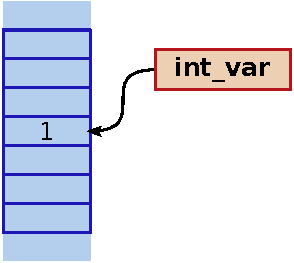
\includegraphics[width=0.23\linewidth]{\currentDir/assignment1}%
\strut\hspace{1.2cm}\strut}%
%
\floatSep%
%
\subfloat[][%
\pythonil{int_var = (3 * int_var) + 1}%
\label{fig:variable:assignment2}%
]{%
\strut\hspace{1.2cm}\strut%
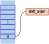
\includegraphics[width=0.23\linewidth]{\currentDir/assignment2}%
\strut\hspace{1.2cm}\strut}%
%
\\%
%
\subfloat[][%
\pythonil{float_var = 3.5}%
\label{fig:variable:assignment3}%
]{%
\strut\hspace{1.2cm}\strut%
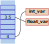
\includegraphics[width=0.23\linewidth]{\currentDir/assignment3}%
\strut\hspace{1.2cm}\strut}%
%
\floatSep%
%
\subfloat[][%
\pythonil{new_var = float_var * int_var}%
\label{fig:variable:assignment4}%
]{%
\strut\hspace{1.2cm}\strut%
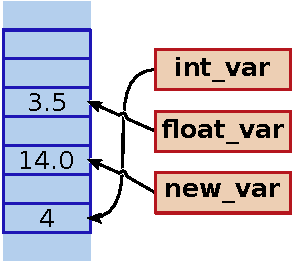
\includegraphics[width=0.23\linewidth]{\currentDir/assignment4}%
\strut\hspace{1.2cm}\strut%
}%
%
\caption{%
Illustrations of the variable assignments in \cref{lst:variables:assignment} in the same order in which they appear in the program: %
Variables are basically names that point to objects which are located somewhere in memory.}%
\label{fig:variable_assignment}%
\end{figure}%
%
\begin{figure}[tb]%
\centering%
%
\subfloat[][%
The file \textil{assignment.py} opened in \pycharm.%
\label{fig:assignmentPyCharm1}%
]{%
\tightbox{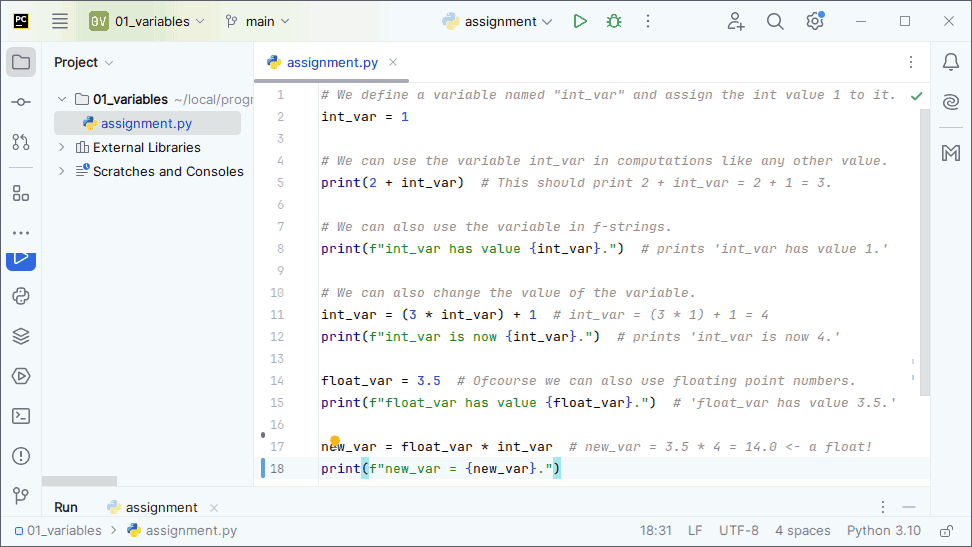
\includegraphics[width=0.49\linewidth]{\currentDir/assignmentPyCharm1}}%
}%
\hfill%
%
\subfloat[][%
Left-clicking on \menu{Run `assignment'} in the pop-up menu after right-clicking on \textil{assignment.py}, or directly pressing \keys{\ctrl+\shift+F10}, to run the program.%
\label{fig:assignmentPyCharm2}%
]{%
\tightbox{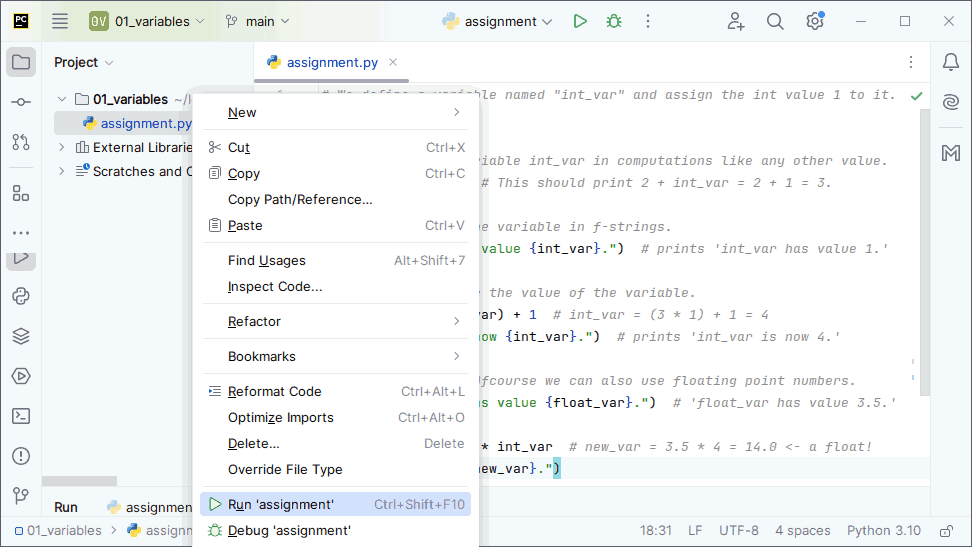
\includegraphics[width=0.49\linewidth]{\currentDir/assignmentPyCharm2}}%
}%
\\%
%
\subfloat[][%
The output of the program \textil{assignment.py} in \pycharm.%
\label{fig:assignmentPyCharm3}%
]{%
\tightbox{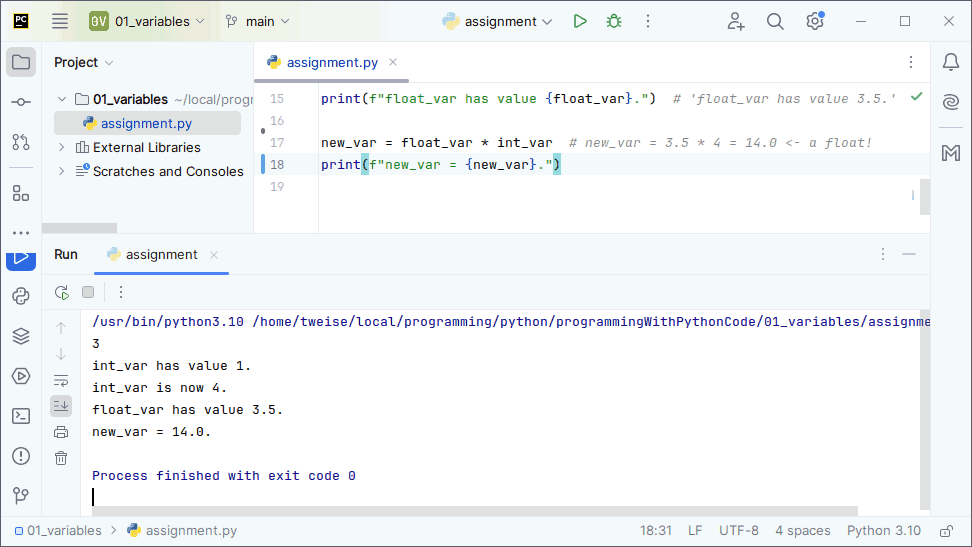
\includegraphics[width=0.7\linewidth]{\currentDir/assignmentPyCharm3}}%
}%
\\%
%
\subfloat[][%
The output of the program \textil{assignment.py} in the \ubuntu\ \pgls{terminal} (which you can open via~\ubuntuTerminal).%
\label{fig:assignmentTerminal}%
]{%
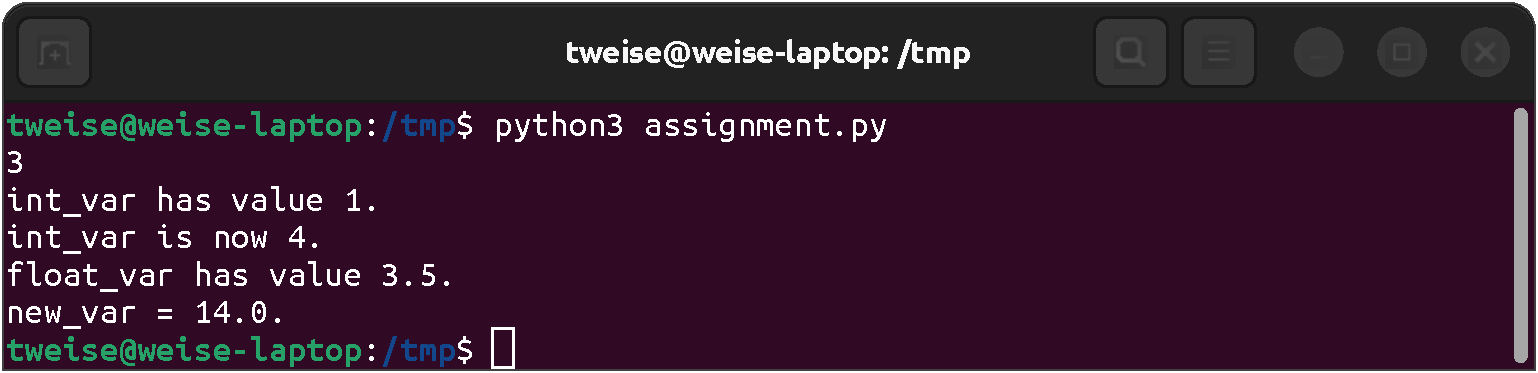
\includegraphics[width=0.7\linewidth]{\currentDir/assignmentTerminal}%
}%
%
\caption{Running the program \textil{assignment.py} from \cref{lst:variables:assignment} in \pycharm~(\cref{fig:assignmentPyCharm1,fig:assignmentPyCharm2,fig:assignmentPyCharm3}) or the \ubuntu\ \pgls{terminal}~(\cref{fig:assignmentTerminal}).}%
\label{fig:variables:assignment}%
\end{figure}%
%
So let's get to the subject of variable assignments with some examples.
\Cref{lst:variables:assignment} shows the source code of our very first commented program.
This program does not do anything useful, but it illustrates how variables can be used.
It begins by assigning the \pythonilIdx{int} value~\pythonil{1} to a variable named~\pythonil{int_var}.
We could have chosen any other name for the variable as well, e.g., \pythonil{my_value}, \pythonil{cow}, \pythonil{race_car}, as long as it does not contain special characters like spaces or line breaks.
But we chose \pythonil{int_var}.
The \pythonilIdx{=} assigns the value~\pythonil{1} to \pythonil{int_value}.
As \cref{fig:variable:assignment1} illustrates, the value~\pythonil{1} will now be stored somewhere in memory and \pythonil{int_var} is a name that points to this memory location.%
%
\begin{sloppypar}%
We can use \pythonil{int_var} just like any other value.
For example, we can compute \pythonil{2 + int_var} and pass the result to the \pythonilIdx{print} function.
This will then print the text~\textil{3} to the \pgls{stdout} of our program.
We can also use \pythonil{int_var} in \pglspl{fstring}\pythonIdx{f-string}\pythonIdx{str!f} about which we learned back in \cref{sec:fstrings}.
\pythonil{f"int_var has value \{int_var\}."} will be \glslink{strinterpolation}{interpolated} to \pythonil{"int_var has value 1."}.%
\end{sloppypar}%
%
Variables are called \emph{variables} and not \emph{constants} because we can change their value.
Hence, we can update \pythonil{int_var} and give it a new value.
For example, we can do \pythonil{int_var = (3 * int_var ) + 1}.
This will update \pythonil{int_var} to now hold the result of the computation \pythonil{(3 * int_var) + 1}.
In this computation, the current (old) value of \pythonil{int_var} is used.
It therefore corresponds to computing \pythonil{(3 * 1) + 1}, which equals~\pythonil{4}.
This value is stored somewhere in memory and \pythonil{int_var} points to it, as sketched in \cref{fig:variable:assignment2}.
The value \pythonil{1} is now no longer referenced.
Eventually, the \python\ interpreter could free the corresponding memory to use it for something else.
Doing \pythonil{print(f"int_var is now \{int_var\}.")} will print \textil{int_var is now 4.} to the \pgls{stdout}.

Of course, we can have multiple variables.
The command \pythonil{float_var = 3.5} creates a variable named \pythonil{float_var}.
It also allocates a piece of memory, writes the floating point value \pythonil{3.5} into it, and lets \pythonil{float_var} point to that piece of memory, as illustrated in \cref{fig:variable:assignment3}.
We can use this variable in an \pgls{fstring}\pythonIdx{f-string}\pythonIdx{str!f} as well:
\pythonil{print(f"float_var has value \{float_var\}.")} is \glslink{strinterpolation}{interpolated} to \pythonil{"float_var has value 3.5."}.%
%
\begin{sloppypar}%
In a final step, we create a third variables with the name \pythonil{new_var} by computing \pythonil{new_var = float_var * int_var}.
The result is \pythonil{3.5 * 4}, i.e., the \pythonilIdx{float} value~\pythonil{14.0}.
\cref{fig:variable:assignment3} illustrates this variable assignment step.
Finally, \pythonil{print(f"new_var = \{new_var\}." )} then prints \textil{new_var = 14.0.}.
(Do you remember a method, to get this output even more easily?)%
\end{sloppypar}%
%
This first program is stored in a file named~\textil{assignment.py}.
To execute it, you have two choices:
You can do this in the \pgls{terminal} or using \pycharm.%
%
\begin{sloppypar}%
Under \ubuntu\ \linux, you open the \pgls{terminal} by pressing \ubuntuTerminal, under \microsoftWindows\ you instead \windowsTerminal.
Then you enter the folder where the program \textil{assignment.py} is stored using the command~\bashil{cd}.
Then you would execute the command~\bashil{python3 assignment.py} to run the \python\ interpreter, as illustrated in \cref{fig:assignmentTerminal}.%
\end{sloppypar}%
%
Alternatively, you can open the program file in \pycharm\ \pgls{ide}, as sketched in \cref{fig:assignmentPyCharm1}.
You would then right-click on the file \textil{assignment.py} in the project tree view.
In the popup-menu that opens, you would left-click on \menu{Run `assignment'} as shown in \cref{fig:assignmentPyCharm2}.
As a shortcut, you can also simply press~\keys{\ctrl+\shift+F10}.
Either way, \pycharm\ will run the program and the output appears in \cref{fig:assignmentPyCharm3}.
As you see, the full \acrfull{stdout} of the complete program given in \cref{exec:variables:assignment} is identical to what we get from the manual execution in either the \pgls{terminal} or \pycharm.

We are not completely done yet, though.
Notice that we wrote the names of variables in a certain style, in lowercase letters.
This is the defactor standard way to name variables and functions in \python\ programming.%
%
\bestPractice{variableNames}{%
Variable names should be lowercase, with words separated by underscores~\cite{PEP8}.%
}
%
This seems like a strange thing to introduce right at the beginning when learning programming.
Matter of fact, we now have seen some best practices on styling our code, e.g., \cref{bp:variableNames,bp:longstrDoubleQuote,bp:comments}, and many more such best practices will follow.
Before continuing further, let us therefore revisit the deeper meaning behind them.
Why is it important to style our code in a consistent way?
Why can't we just write things down in any way that pleases us?

Well, because following best practices is nothing that can be done \inQuotes{later.}
You will never have the time to revisit and improve the style of your old code.
It is also nothing that you can just switch over to.
If you have learned doing a certain thing in a certain way, it will always be hard to switch over to a different way.
If an apprentice in a kitchen is not taught to wash their hands before beginning to prepare meals, then they will not simply begin doing that consistently after being told to do it once after they join a new restaurant.
Following style guides and best practices is a habit.
And we need to nurture this habit right from the start.%
%
\bestPractice{codeStyle}{%
Regardless which programming language you are using, it is important to write code and scripts in a consistent style, to use a consistent naming scheme for all things that can be named, and to follow the generally established best practices and norms for that language.%
}%
%
For many programming languages, there exist comprehensive and clear style guides.
Since we usually work collaboratively on larger projects, writing code in a consistent style is very important.
Ideally, all collaborators can open a source code file and easily read and understand our code.
If everybody writes code in different styles, maybe using different indentations or different naming conventions, reading code can become harder and even confusing.
Therefore, style guides often tell us how to name things and how to structure code consistently.%
%
\bestPractice{PEP8}{%
The most important style guide for the \python\ programming language is PEP8:~\citetitle{PEP8}~\cite{PEP8} at \citeurl{PEP8}. %
\python\ code violating PEP8 is invalid \python code.%
}%
%
\FloatBarrier%
\endhsection%
%
\hsection{LIU Hui's Method for the Approximation of~$\numberPi$}%
\label{sec:approximatePiLiuHui}%
%
\begin{figure}%
\centering%
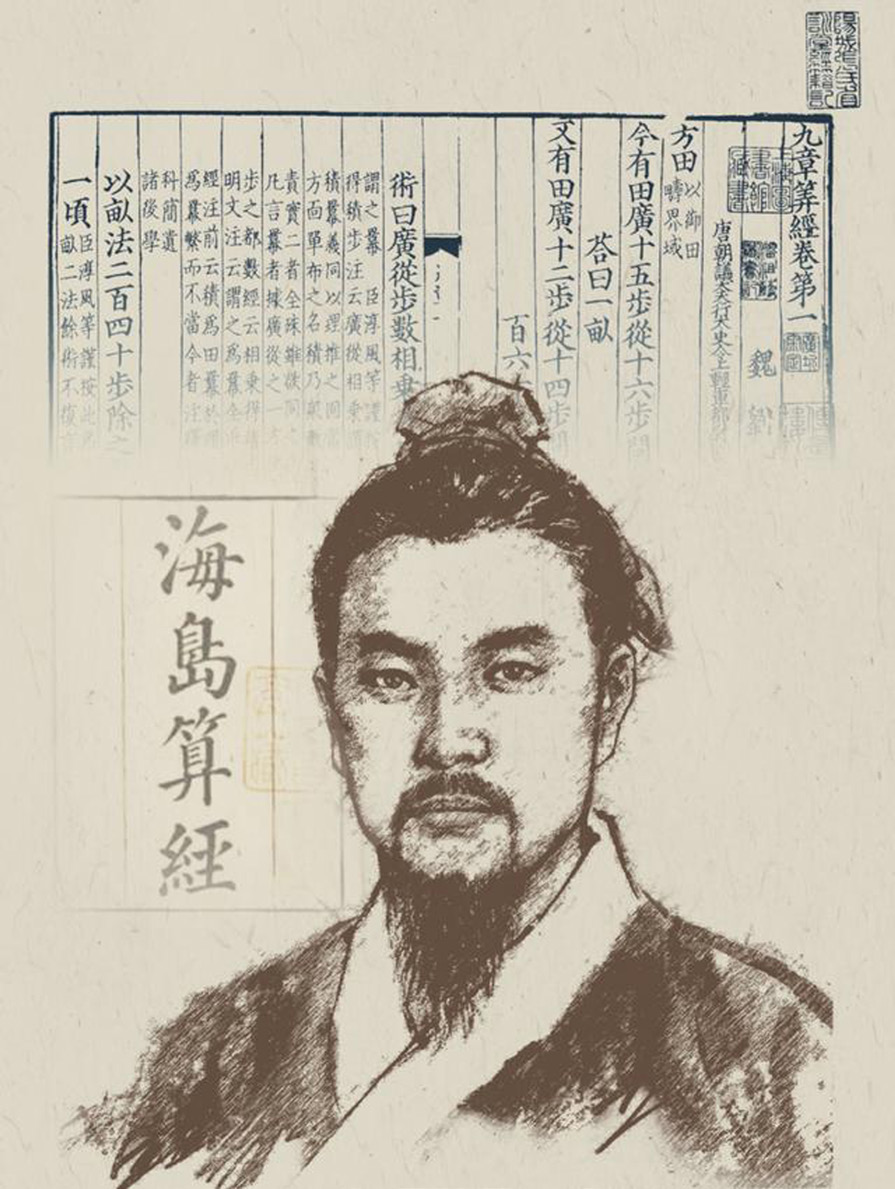
\includegraphics[width=0.3\linewidth]{\currentDir/liu_hui.jpg}%
\caption{Modern rendition of LIU Hui~(刘徽) from~\cite{Y2024COACMMLHFHTIOMACE}. %
Not under the Creative Commons license, copyright~\textcopyright\ is with CAST / Official WeChat account of VOC.}%
\label{fig:liu_hui}%
\end{figure}%
%
\begin{figure}%
\centering%
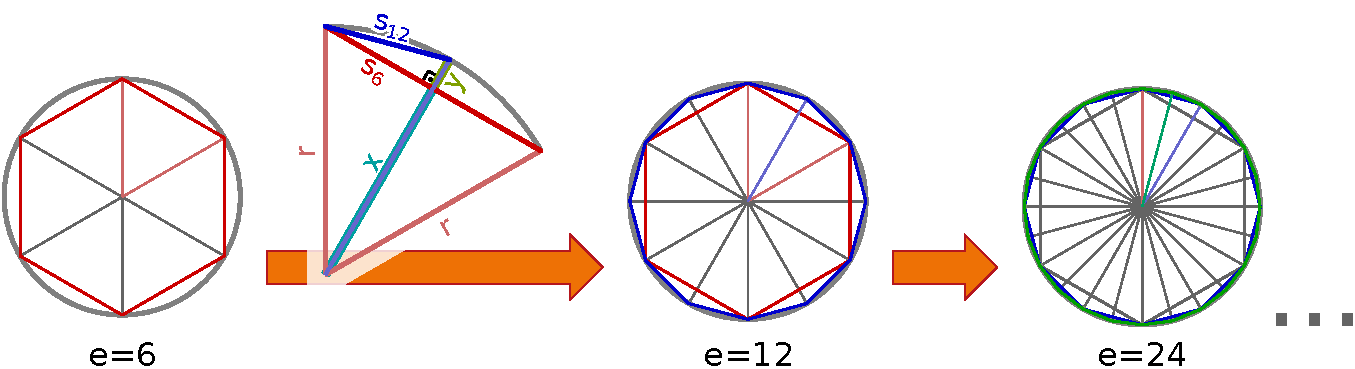
\includegraphics[width=0.99\linewidth]{\currentDir/liuHuiCircle}%
\caption{Approximating the ratio of the circumference and the diameter of a circle, i.e., $\numberPi$, by inscribing regular~$3*2^n$-gons.}%
\label{fig:liuHuiCircle}%
\end{figure}%
%
\definecolor{liuhui-r-color}{HTML}{CC6666}%
\def\liuhuir{\ensuremath{{\color{liuhui-r-color}r}}}%
\definecolor{liuhui-s6-color}{HTML}{CC0000}%
\def\liuhuiss{\ensuremath{{\color{liuhui-s6-color}s_6}}}%
\definecolor{liuhui-s12-color}{HTML}{0000CC}%
\def\liuhuist{\ensuremath{{\color{liuhui-s12-color}s_{12}}}}%
\definecolor{liuhui-y-color}{HTML}{80A000}%
\def\liuhuiy{\ensuremath{{\color{liuhui-y-color}y}}}%
\definecolor{liuhui-x-color}{HTML}{00A0A0}%
\def\liuhuix{\ensuremath{{\color{liuhui-x-color}x}}}%
\definecolor{liuhui-s24-color}{HTML}{00A000}%
\def\liuhuistf{\ensuremath{{\color{liuhui-s24-color}s_{24}}}}%
%
Let us now come to a more serious example.
I am not good at mathematics, but I still really like mathematics anyway, so we will go with a mathematics example: approximating~\numberPi.
The number~\numberPi\ is the ratio of the circumference of a circle and its diameter.
A we already mentioned before in \cref{sec:float}, it is transcendental, a never-ending and never-repeating sequence of digits.
We can compute it to a certain precision, e.g., as the \pythonilIdx{float} constant \pythonilIdx{pi} with value \pythonil{3.141592653589793}.
But we can never really write it down in its entirety.

Well, when I say \inQuotes{we can compute it}, then the question \inQuotes{How?} immediately arises.
One particularly ingenious answer was given by the Chinese mathematician LIU Hui~(刘徽, who may have looked as sketched \cref{fig:liu_hui}) somewhere in the third century~\pgls{CE}~\cite{OR2003LH,Y2024COACMMLHFHTIOMACE} in his commentary to the famous Chinese mathematics book \emph{Jiu Zhang Suanshu}~(九章算术)~\cite{OR2003LH,SCL1999TNCOTMACAC,S1998LHATFGAOCM,D2010AALHOCAS,C2002LFLHADWTDM}.
In \cref{fig:liuHuiCircle}, we show how~\numberPi\ can be approximated based on the idea of LIU Hui~(刘徽):
By inscribing regular~$e$\nobreakdashes-gons with an increasing number~$e$ of edges into a circle such that the corners of the $e$\nobreakdashes-gons lie on the circle.

We start with a hexagon~($e=6$) where the radius~\liuhuir\ is equal to the radius of the circle.
Since it is a regular hexagon, it can be divided into six triangles.
These are isosceles triangle, since two sides of each triangle have length~\liuhuir, since two of its edges are on the cirlce and the third edge is the circle center.
The apex angle between these two eges is~$60^{\circ}$, as $360^{\circ}/6=60^{\circ}$.
Therefore, the triangles are equilateral, meaning that the third side also has length~\liuhuir.

This means that all the $e$~edges~\liuhuiss\ of this hexagon then have length~\liuhuir\ as well.
It is easy to see that the circumference of the hexagon is~$U=e*\liuhuiss=6*\liuhuir$.
The diameter of the circle is~$D=2\liuhuir$.
Assuming that the circumference of the hexagon is an approximation of the circumference of the circle, we could approximate~\numberPi\ as $\numberPi\approx\frac{U}{D}$.
For $e=6$~edges, this gives us $\numberPi_6=\frac{6\liuhuir}{2\liuhuir}=3$.

Now this is a very coarse approximation of~\numberPi.
We can get closer to the actual ratio if we would use more edges, i.e., higher values of~$e$.
The ingenious idea of LIU Hui~(刘徽) is to use $e$\nobreakdashes-gons with~$e=3*2^n$.
For $n=1$, we get the hexagon with $e=6$.
For $n=2$, we double the edges and have a dodecagon with $e=12$~edges.
But how do we get the edge length~\liuhuist\ of this dodecagon?

We can get it from the edge length~\liuhuiss\ and radius~\liuhuir\ of the hexagon.
If we use the same six corners for the hexagon and dodecagon and connect the newly added six corners with the center of the circle, then these connections will separate each edge of the hexagon exactly in half and do so at a $90^\circ$~angle, as shown again in \cref{fig:liuHuiCircle}.
Here, the new side length~\liuhuist\ is the hypotenuse of a right-angled triangle with base~$\frac{\liuhuiss}{2}$ and height~\liuhuiy.
To get the height~\liuhuiy, we can use that~$\liuhuir=\liuhuix+\liuhuiy$ and the fact that there is a second right-angled triangle here, namely the one with base~\liuhuix, height~$\frac{\liuhuiss}{2}$, and hypotenuse~\liuhuir.
This gives us $\liuhuix^2+\left(\frac{\liuhuiss}{2}\right)^2=\liuhuir^2$.
Let's make things easier by choosing~$\liuhuir=1$.

We get $\liuhuix^2=1-\left(\frac{\liuhuiss}{2}\right)^2=1-\frac{\liuhuiss^2}{4}$ and, hence, $\liuhuiy=1-\sqrt{1-\frac{\liuhuiss^2}{4}}$.
With this we can move on to $\liuhuist^2=\liuhuiy^2+\left(\frac{\liuhuiss}{2}\right)^2$, which we can resolve to $\liuhuist^2=\left(1-\sqrt{1-\frac{\liuhuiss^2}{4}}\right)^2+\frac{\liuhuiss^2}{4}$.
Using $(a-b)^2=a^2-2ab+b^2$ and applying it to the first term, we get $\liuhuist^2=1-2\sqrt{1-\frac{\liuhuiss^2}{4}}+\left(1-\frac{\liuhuiss^2}{4}\right)+\frac{\liuhuiss^2}{4}$.
This then gives us $\liuhuist^2=2-2\sqrt{1-\frac{\liuhuiss^2}{4}}-\frac{\liuhuiss^2}{4}+\frac{\liuhuiss^2}{4}$, which we can further refine to $\liuhuist^2=2-2\sqrt{1-\frac{\liuhuiss^2}{4}}$.
We can pull the~$2$ from outside the root into the root by multiplying everything inside by $2^2=4$ and get $\liuhuist^2=2-\sqrt{4-\liuhuiss^2}$.
Thus, we have the really elegant $\liuhuist=\sqrt{2-\sqrt{4-\liuhuiss^2}}$.

As new approximation of~$\numberPi_{12}$, we now have $\frac{12*\liuhuist}{2\liuhuir}=6*\liuhuist=6\sqrt{2-\sqrt{4-\liuhuiss^2}}=6\sqrt{2-\sqrt{4-1}}=6\sqrt{2-\sqrt{3}}\approx 3.105828539$.
This is already quite nice.
We can actually repeat this step to get to~\liuhuistf.
And we could continue this process by again doubling the number the edges.
Repeating the above calculations and observing \cref{fig:liuHuiCircle}, we get the equation:%
%
\begin{align}%
s_{2e} &= \sqrt{2-\sqrt{4-s_e^2}}\label{eq:liuhui:sidelength}\\%
\numberPi_{2e} &= \frac{e}{2} s_{2e}\label{eq:liuhui:approx}%
\end{align}%
%
\gitLoadAndExecPython{variables:pi_liu_hui}{}{variables}{pi_liu_hui.py}{}%
\listingPythonAndOutput{variables:pi_liu_hui}{%
A \python\ program showing several steps of the approximation of~\numberPi\ using the method of LIU Hui~(刘徽).}{}%
%
\begin{figure}[tb]%
\centering%
%
\subfloat[][%
The file \programUrl{variables:pi_liu_hui} opened in \pycharm.%
\label{fig:liuHuiPiPyCharm1}%
]{%
\tightbox{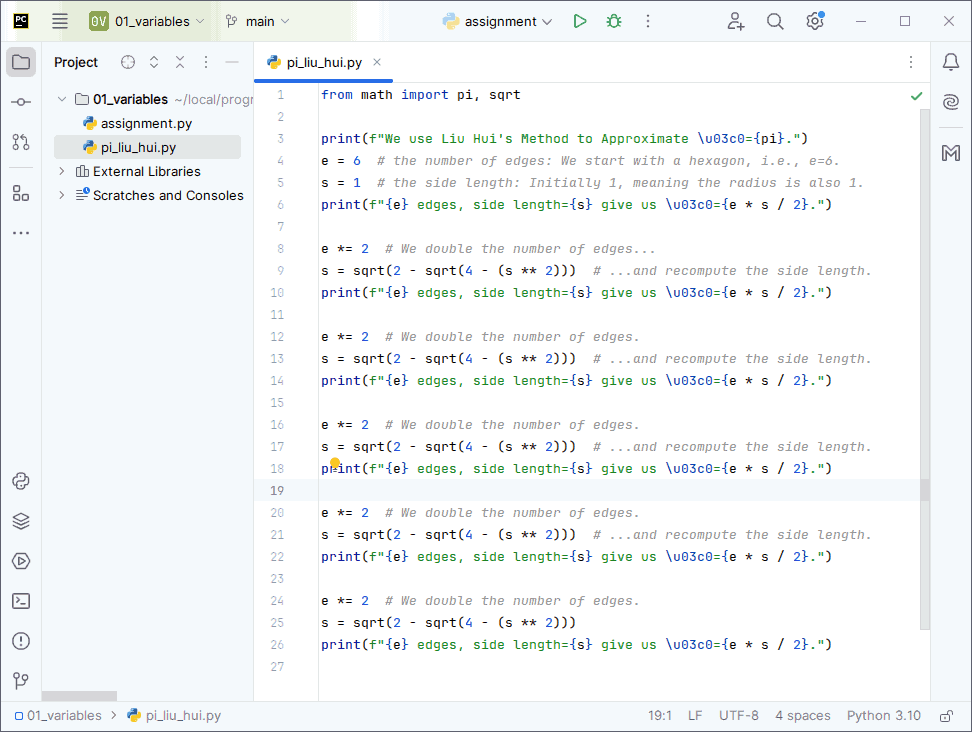
\includegraphics[width=0.49\linewidth]{\currentDir/liuHuiPiPyCharm1}}%
}%
\hfill%
%
\subfloat[][%
Left-clicking on \menu{Run `pi\_liu\_hui'} in the pop-up menu after right-clicking on \programUrl{variables:pi_liu_hui}, or directly pressing \keys{\ctrl+\shift+F10}, to run the program.%
\label{fig:liuHuiPiPyCharm2}%
]{%
\tightbox{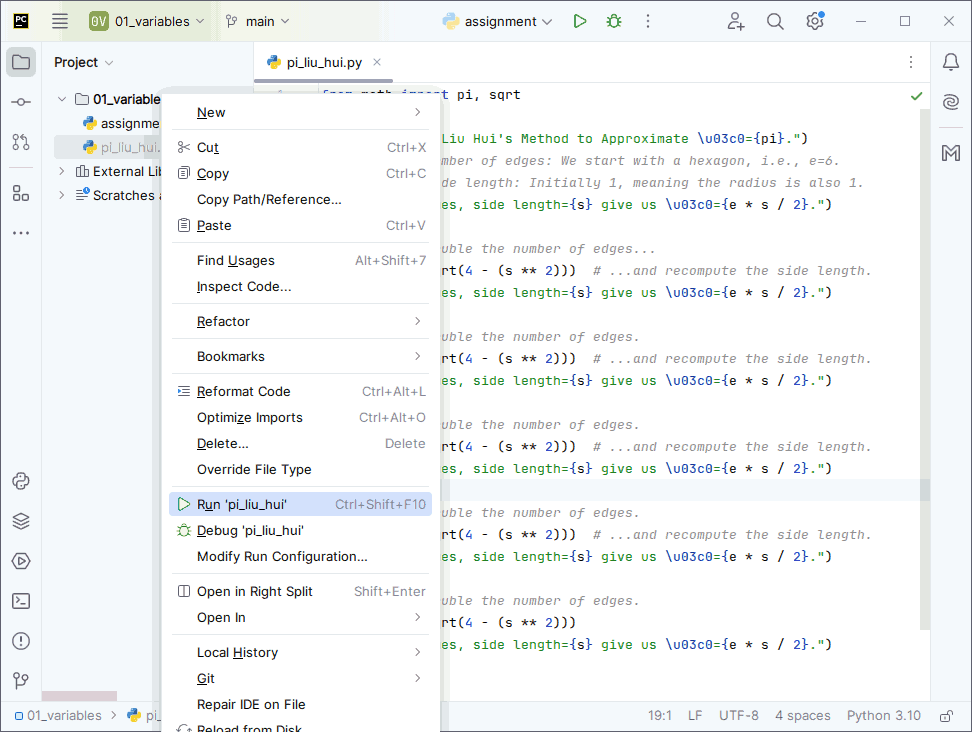
\includegraphics[width=0.49\linewidth]{\currentDir/liuHuiPiPyCharm2}}%
}%
\\%
%
\subfloat[][%
The output of the program \programUrl{variables:pi_liu_hui} in \pycharm.%
\label{fig:liuHuiPiPyCharm3}%
]{%
\tightbox{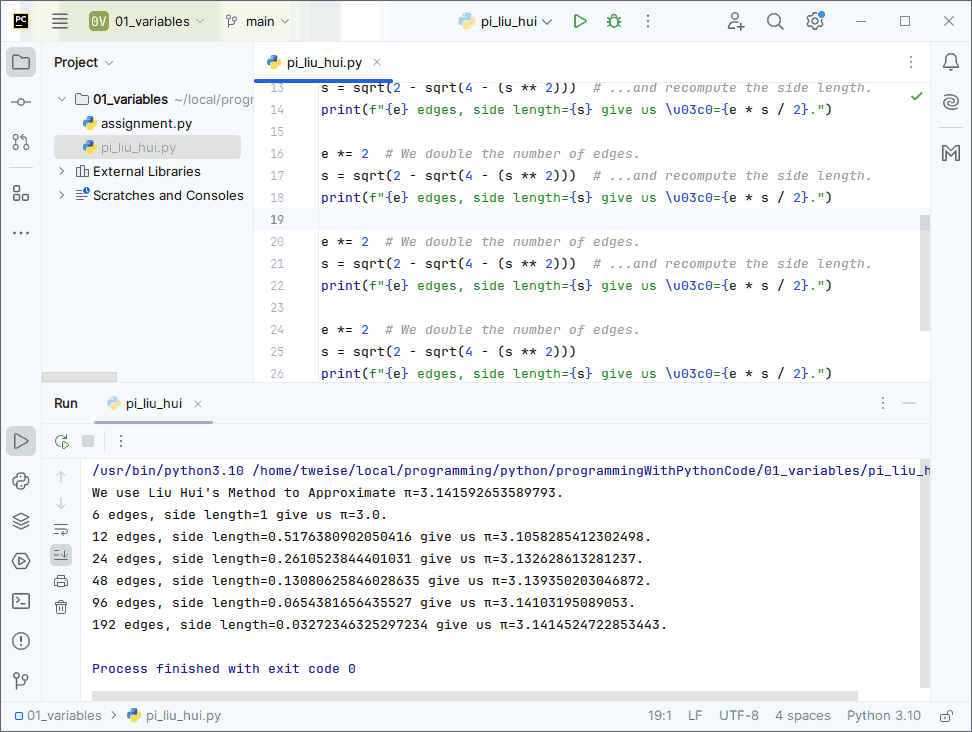
\includegraphics[width=0.7\linewidth]{\currentDir/liuHuiPiPyCharm3}}%
}%
\\%
%
\subfloat[][%
The output of the program \programUrl{variables:pi_liu_hui} in the \ubuntu\ \pgls{terminal} (which you can open via~\ubuntuTerminal).%
\label{fig:liuHuiPiTerminal}%
]{%
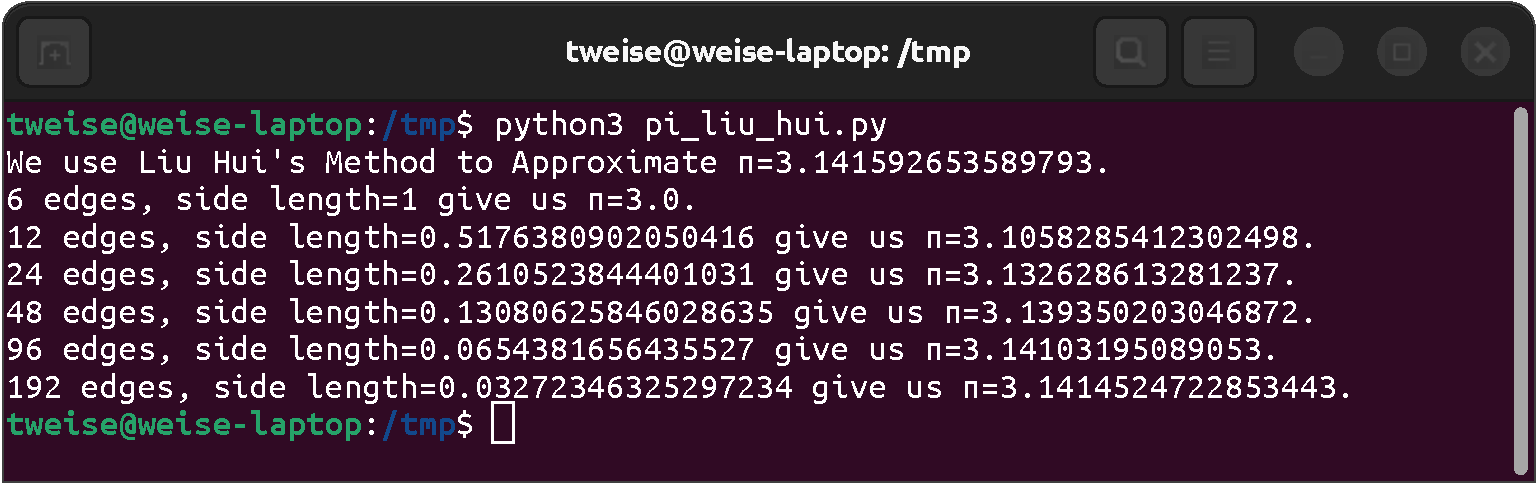
\includegraphics[width=0.7\linewidth]{\currentDir/liuHuiPiTerminal}%
}%
%
\caption{Running the program \programUrl{variables:pi_liu_hui} from \cref{lst:variables:assignment} in \pycharm~(\cref{fig:liuHuiPiPyCharm1,fig:liuHuiPiPyCharm2,fig:liuHuiPiPyCharm3}) or the \ubuntu\ \pgls{terminal}~(\cref{fig:liuHuiPiTerminal}).}%
\label{fig:variables:liuHuiPi}%
\end{figure}%
%
Now that we have learned some programming, we do no longer need to type the numbers and computation steps into a calculator.
We also do not need to use \python\ as calculator.
Instead, we can enter all the commands needed for the computation into a program file.
We will call it~\textil{pi_liu_hui.py}, as illustrated in \cref{lst:variables:pi_liu_hui}.

We begin by setting the initial number of edges \pythonil{e = 6} and the initial side length of the $e$\nobreakdashes-gon to \pythonil{s = 1}, because we still keep with the choice of~$\liuhuir=1$.
In each iteration of the approximation, we simply set \pythonil{e *= 2}\pythonIdx{*=}, which is equivalent to \pythonil{e = e * 2}, to double the number of edges.
We compute \pythonil{s = sqrt(2 - sqrt(4 - (s ** 2)))}\pythonIdx{sqrt} having imported\pythonIdx{import} the \pythonilIdx{sqrt} function from the \pythonilIdx{math} module.
We print the approximated value of~\numberPi\ as \pythonil{e * s / 2}.
Notice how elegantly we use the \pgls{unicode} characters~$\pi$ and~$\approx$ via the \pglspl{escapeSequence}~\pythonil{\\u03c0} and \pythonil{\\u2248}\pythonIdx{\textbackslash{u}}, respectively, from back in~\cref{sec:unicodeChars} (and how nicely it indeed prints the greek character~$\pi$ in the \pgls{stdout} in \cref{exec:variables:pi_liu_hui}).
Either way, since \cref{eq:liuhui:sidelength,eq:liuhui:approx} are always the same, we can simply copy-paste the lines of code for updating~\pythonil{s}, \pythonil{e}, and printing the approximated value of~\numberPi\ several times.

\Cref{exec:variables:pi_liu_hui} shows the \acrfull{stdout} produced by this program.
Indeed, each new approximation comes closer to~\numberPi.
For 192~edges, we get the approximation~\pythonil{3.1414524722853443}.
Given that the constant~\pythonilIdx{pi} from the \pythonilIdx{math} module is \pythonil{3.141592653589793}, we find that the first four digits are correct and that the number is only off by only 0.0045\%!

For your convenience, we also showed the results when executing the program in \pycharm\ or the \ubuntu\ \pgls{terminal} in \cref{fig:variables:liuHuiPi}.
To open a \pgls{terminal} under \ubuntu\ \linux, you would press~\ubuntuTerminal, whereas under \microsoftWindows, you~\windowsTerminal.
With the command \bashil{cd}, you would enter the directory where our program \textil{pi_liu_hui.py} is located.
You would then type in \bashil{python3 pi_liu_hui.py} and hit~\keys{\enter}.
As you can see in \cref{fig:liuHuiPiTerminal}, you will get the same output as given in \cref{exec:variables:pi_liu_hui}.

Alternatively, if you are using \pycharm, you can open the program file \programUrl{variables:pi_liu_hui} as shown in \cref{fig:liuHuiPiPyCharm1}.
You can right-click on this program in the project tree view and, in the pop-up menu that appears, left-click on \menu{Run `pi\_liu\_hui'}, as sketched in \cref{fig:liuHuiPiPyCharm2}.
You can instead also press \keys{\ctrl+\shift+F10} in the editor window.
Either way, the program will be executed and its output appears~(see~\cref{fig:liuHuiPiPyCharm3}).
And again it is identical to what we have shown in \cref{exec:variables:pi_liu_hui}.
Therefore, in the future, we will only very sporadically add such screenshots.
Instead, we will usually only print code and output pairs like~\cref{lst:variables:pi_liu_hui,exec:variables:pi_liu_hui}.%
%
\endhsection%
%
\hsection{Summary}%
%
We now have learned how we can store values in variables.
We also have learned that we can then use the variables instead of the values.
We further have learned that we can assign new values to variables and do so multiple times.

This means that we can now, for the first time, create meaningful programs consisting of multiple lines of code.
Programs, in which the intermediate results computed by one line of code are transmitted and used in a later line of code.
This is a huge jump.

Now our code can become much more complex.
This means that we must now begin to consider issues such as code quality.
We need to follow style guides to make the code readable.
We need to write comments into our code, so that we~(and others) can later understand what we were thinking when writing the programs.

But most importantly:
We can already do some cool stuff!%
\endhsection%
%
\FloatBarrier%
\endhsection%
%
